\chapter{ポアソン括弧、生成子、角運動量}

\lectureoverview{ポアソン括弧は、ハミルトンの方程式を書き直すための簡潔な方法以上のものである。それは変換を生成する代数的操作である。ハミルトニアンとの括弧は時間発展を生成し、運動量との括弧は並進を生成し、角運動量との括弧は回転を生成する。この言葉遣いでは、対称性と保存則は、一つの消える括弧の二つの読み方になる。この考えを調和振動子から展開し、次に角運動量代数を用いて、オイラー角を導入することなくジャイロスコープの歳差運動を得る。}

\section{ハミルトン軌道に沿った関数}

\[
  F=F(q_1,\ldots,q_n,p_1,\ldots,p_n)
\]を相空間上の十分に微分可能な関数とする。これは二つの仕方で見ることができる。第一に、相空間の各点に数を割り当てる。第二に、ハミルトン軌道が一つ選ばれると、点\((q(t),p(t))\)が動くので、時間の関数になる。その軌道に沿って、\begin{equation}
  \frac{dF}{dt}
  =
  \sum_i\left(
    \frac{\partial F}{\partial q_i}\dot q_i
    +\frac{\partial F}{\partial p_i}\dot p_i
  \right).
  \label{eq:l8-chain-rule}
\end{equation}ハミルトンの方程式\begin{equation}
  \dot q_i=\frac{\partial H}{\partial p_i},
  \qquad
  \dot p_i=-\frac{\partial H}{\partial q_i},
  \label{eq:l8-hamilton-equations}
\end{equation}はこれを\begin{equation}
  \frac{dF}{dt}
  =
  \sum_i\left(
    \frac{\partial F}{\partial q_i}
    \frac{\partial H}{\partial p_i}
    -
    \frac{\partial F}{\partial p_i}
    \frac{\partial H}{\partial q_i}
  \right).
  \label{eq:l8-fdot-expanded}
\end{equation}に変える。右辺の組み合わせは、その二つの要素のどちらもハミルトニアンでない場合でさえ、古典力学の至るところに現れる。このことが定義\begin{equation}
  \boxed{
  \{F,G\}
  =
  \sum_i\left(
    \frac{\partial F}{\partial q_i}
    \frac{\partial G}{\partial p_i}
    -
    \frac{\partial F}{\partial p_i}
    \frac{\partial G}{\partial q_i}
  \right).}
  \label{eq:l8-poisson-definition}
\end{equation}を動機づける。したがって式~\eqref{eq:l8-fdot-expanded}は\begin{equation}
  \boxed{\dot F=\{F,H\}.}
  \label{eq:l8-time-generator}
\end{equation}となる。

\begin{classroomqa}
  \audiencequestion{第二の要素を\(H\)から任意の関数\(G\)に変えたとき、括弧は依然として\(F\)の時間微分であるか。
  \lecturetimestamp{00:05:45--00:06:15}}
  \lecturerresponse{いいえ。記法が一般化されるにつれて、聴衆は重要な点を捉える。式~\eqref{eq:l8-poisson-definition}は任意の二つの相空間関数に対して\(\{F,G\}\)を定義するが、\(\dot F=\{F,G\}\)は\(G\)がハミルトニアンであるときにのみ成り立つ。一般の\(G\)は異なる無限小変換を生成するであろう。}
\end{classroomqa}

時間の微小変化を\begin{equation}
  \delta_t F=\epsilon\,\{F,H\}.
  \label{eq:l8-small-time-step}
\end{equation}と書くと有用である。この形は後に来るものを予期している。時間発展は、ポアソン括弧によって生成されるより大きな変換族の一員である。

\section{括弧の代数}

この括弧は今やそれ自体の計算として用いることができる。その規則は通常の微分から従う：\begin{align}
  \{A,B\}&=-\{B,A\}, \label{eq:l8-antisymmetry}\\
  \{A+B,C\}&=\{A,C\}+\{B,C\}, \label{eq:l8-additivity}\\
  \{\lambda A,B\}&=\lambda\{A,B\},
    \quad \lambda\ \text{constant}, \label{eq:l8-scalar-rule}\\
  \{AB,C\}&=A\{B,C\}+\{A,C\}B. \label{eq:l8-leibniz}
\end{align}これら四行は、それぞれ反対称性、加法性、定数倍に関する線形性、ライプニッツ則を表す。古典的な相空間関数は可換に掛け合わされるので、最後の行における通常の因子\(A\)と\(B\)の位置は重要でない。そのことは量子力学における演算子に対してはもはや成り立たない。反対称性はまた\begin{equation}
  \{A,A\}=0.
  \label{eq:l8-self-bracket}
\end{equation}を意味する。

正準座標に対して、基本括弧は\begin{equation}
  \boxed{
  \{q_i,q_j\}=0,\qquad
  \{p_i,p_j\}=0,\qquad
  \{q_i,p_j\}=\delta_{ij}.}
  \label{eq:l8-canonical-brackets}
\end{equation}である。\(q_i\)のみの任意の関数は、\(q_i\)のみの任意の他の関数とゼロの括弧をもつ。同様のことが\(p_i\)のみの関数についても成り立つ。非零の括弧には、正準座標がその共役運動量と出会うことが必要である。式~\eqref{eq:l8-canonical-brackets}のクロネッカーのデルタは、一致する添字だけが出会うことを記録している。

\subsection{試験としての調和振動子}

\begin{equation}
  H=\frac{p^2}{2m}+\frac{kq^2}{2}.
  \label{eq:l8-oscillator-hamiltonian}
\end{equation}を考える。ここでは意図的に括弧の規則と式~\eqref{eq:l8-time-generator}のみを用いる。第一に、\begin{align}
  \dot q
  &=\{q,H\}\\
  &=\frac{1}{2m}\{q,p^2\}\\
  &=\frac{1}{2m}\left(p\{q,p\}+\{q,p\}p\right)\\
  &=\frac{p}{m}.
  \label{eq:l8-qdot-oscillator}
\end{align}ポテンシャル項は\(\{q,q^2\}=0\)のために消える。同様に、\begin{align}
  \dot p
  &=\{p,H\}\\
  &=\frac{k}{2}\{p,q^2\}\\
  &=\frac{k}{2}\left(q\{p,q\}+\{p,q\}q\right)\\
  &=-kq.
  \label{eq:l8-pdot-oscillator}
\end{align}マイナス符号はまさに反対称性\(\{p,q\}=-\{q,p\}=-1\)である。二つの一階方程式を組み合わせると\begin{equation}
  m\ddot q=-kq.
  \label{eq:l8-hooke-equation}
\end{equation}が得られる。

\begin{figure}[htbp]
  \centering
  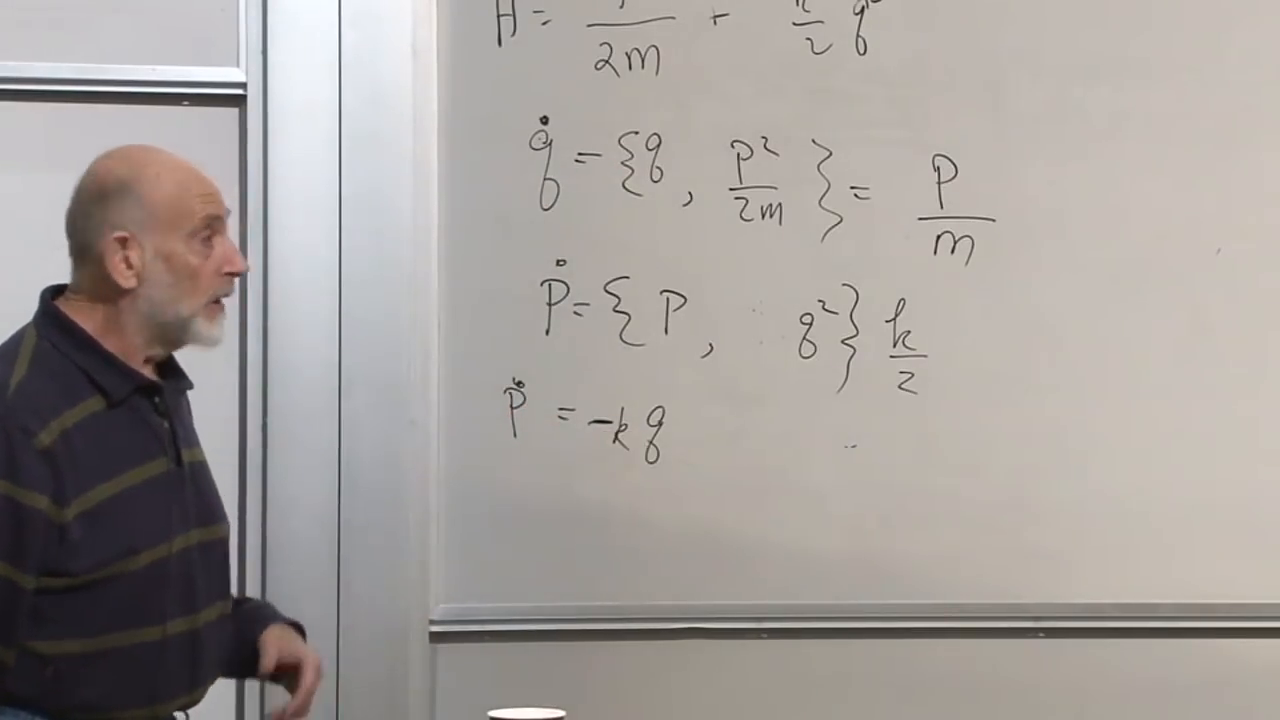
\includegraphics[width=0.82\textwidth]{lecture_08_figure_01.png}
  \caption{振動子のハミルトニアンと、\(\dot q=p/m\)および\(\dot p=-kq\)を与える二つの括弧計算。}
  \lectureframe{00:23:20}
\end{figure}

計算の間、クラスは\emph{ポアソン括弧を取る}という意味の動詞を探し、暫定的に\emph{ポアソンする}に落ち着く。この冗談は視点の実際の変化を示している。すなわち、代数が分かれば、すべての結果を定義から再導出する代わりに、それを直接扱うことができる。

\begin{classroomqa}
  \audiencequestion{この数学的構造は群か、それとも代数か。逆元をもつか。\lecturetimestamp{00:23:48--00:24:16}}
  \lecturerresponse{群ではない。括弧演算は必要な単位元と逆元を与えない。相空間関数はポアソン代数をなす。すなわち、通常の可換な乗法と加法、およびライプニッツ則を満たす反対称な括弧をもつ。さらなる恒等式であるヤコビ恒等式が通常の抽象的定義を完成させるが、それはこの講義では展開されない。}
\end{classroomqa}

\begin{classroomqa}
  \audiencequestion{ポアソン括弧と量子交換子の間にはどのような関係があるのか。\lecturetimestamp{00:24:18--00:25:00}}
  \lecturerresponse{この講義では予備的な説明のみを行う。量子力学への移行において、古典的な括弧は模式的に次で置き換えられる。
  \[
    \{A,B\}_{\mathrm{PB}}
    \longleftrightarrow
    \frac{1}{i\hbar}[\widehat A,\widehat B].
  \]
  この対応には演算子の順序と量子化に関する但し書きが必要であり、ここでは定理として用いているわけではない。}
\end{classroomqa}

振動子の場合、この括弧は単にハミルトンの方程式を再構成したにすぎない。その真の経済性は、生成子が\(H\)以外の保存量であるときに現れる。

\section{回転対称性から角運動量を再導出する}

以前の講義で用いたネーターの構成法の無限小形を思い出そう。連続対称性が座標を
\begin{equation}
  \delta q_i=\epsilon F_i(q),
  \label{eq:l8-noether-variation}
\end{equation}
だけ変化させるならば、ここで考察している設定では、その保存量は
\begin{equation}
  G=\sum_i p_iF_i(q).
  \label{eq:l8-noether-charge}
\end{equation}
である。全体の因子\(\epsilon\)は省略してよい。保存量に固定した数を掛けても保存則は変わらないからである。

1個の粒子を取り、\(z\)軸のまわりに無限小回転させる。講義で用いた向きでは、
\begin{equation}
  \delta x=-\epsilon y,\qquad
  \delta y=\epsilon x,\qquad
  \delta z=0.
  \label{eq:l8-z-rotation}
\end{equation}
式~\eqref{eq:l8-noether-charge}より
\begin{equation}
  L_z=-p_xy+p_yx=xp_y-yp_x.
  \label{eq:l8-lz}
\end{equation}
\(x\)、\(y\)、\(z\)について巡回的に繰り返すと、
\begin{equation}
  \boxed{\begin{aligned}
    L_x&=yp_z-zp_y,\\
    L_y&=zp_x-xp_z,\\
    L_z&=xp_y-yp_x.
  \end{aligned}}
  \label{eq:l8-angular-components}
\end{equation}
これらは
\begin{equation}
  \boldsymbol L=\boldsymbol r\times\boldsymbol p.
  \label{eq:l8-cross-product}
\end{equation}
の成分である。

\begin{figure}[htbp]
  \centering
  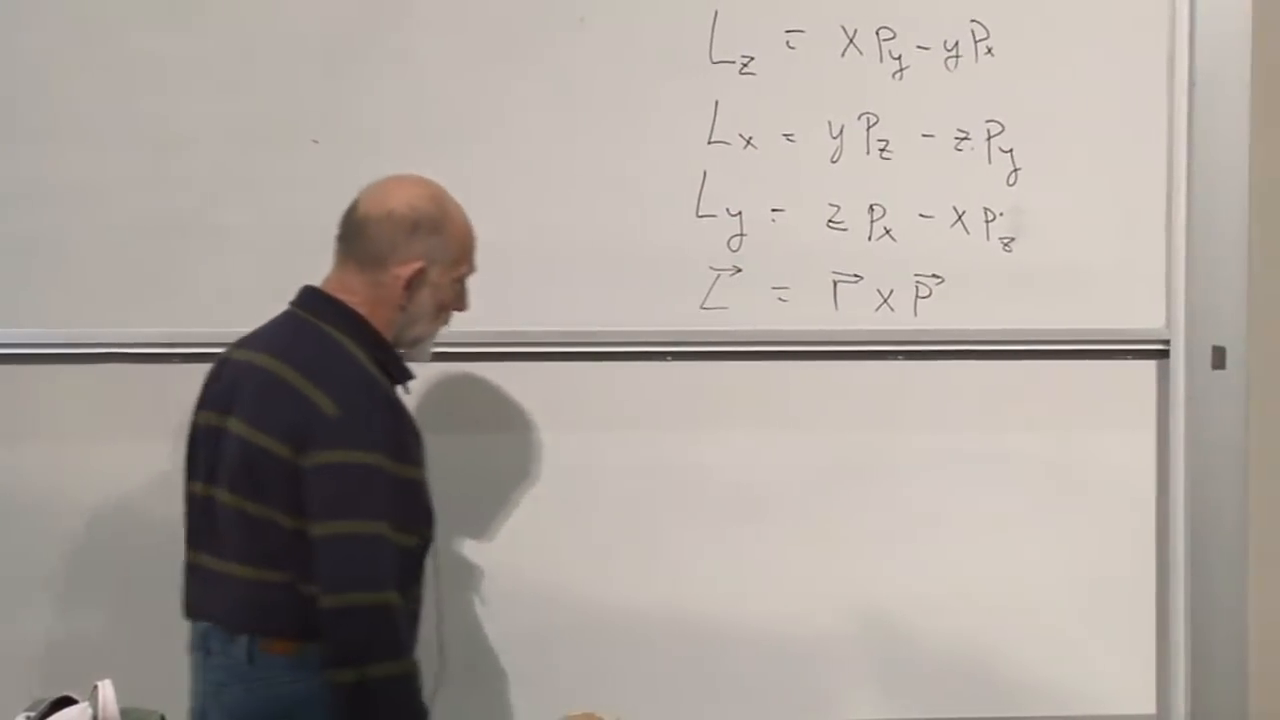
\includegraphics[width=0.82\textwidth]{lecture_08_figure_02.png}
  \caption{角運動量の3つのデカルト成分と、それらの簡潔な外積形。}
  \lectureframe{00:34:00}
\end{figure}

任意の単位ベクトル\(\boldsymbol n\)のまわりの回転は
\begin{equation}
  L_{\boldsymbol n}=\boldsymbol n\cdot\boldsymbol L.
  \label{eq:l8-arbitrary-axis}
\end{equation}
によって生成される。孤立した回転不変系では、3つの成分すべてが保存される。1つの軸のまわりの回転のみが対称性として残る場合、その軸に沿った成分のみが保存を保証される。

\section{角運動量が回転を生成する}

回転力学の問題を直ちに解く代わりに、\(L_z\)が括弧の下で何を行うかを調べよう。式~\eqref{eq:l8-lz}を用いると、
\begin{align}
  \{x,L_z\}
  &=\{x,xp_y-yp_x\}
   =-y\{x,p_x\}
   =-y,\\
  \{y,L_z\}
  &=\{y,xp_y-yp_x\}
   =x\{y,p_y\}
   =x,\\
  \{z,L_z\}&=0.
  \label{eq:l8-position-rotation-brackets}
\end{align}
これらは式~\eqref{eq:l8-z-rotation}の係数にほかならない。

\begin{figure}[htbp]
  \centering
  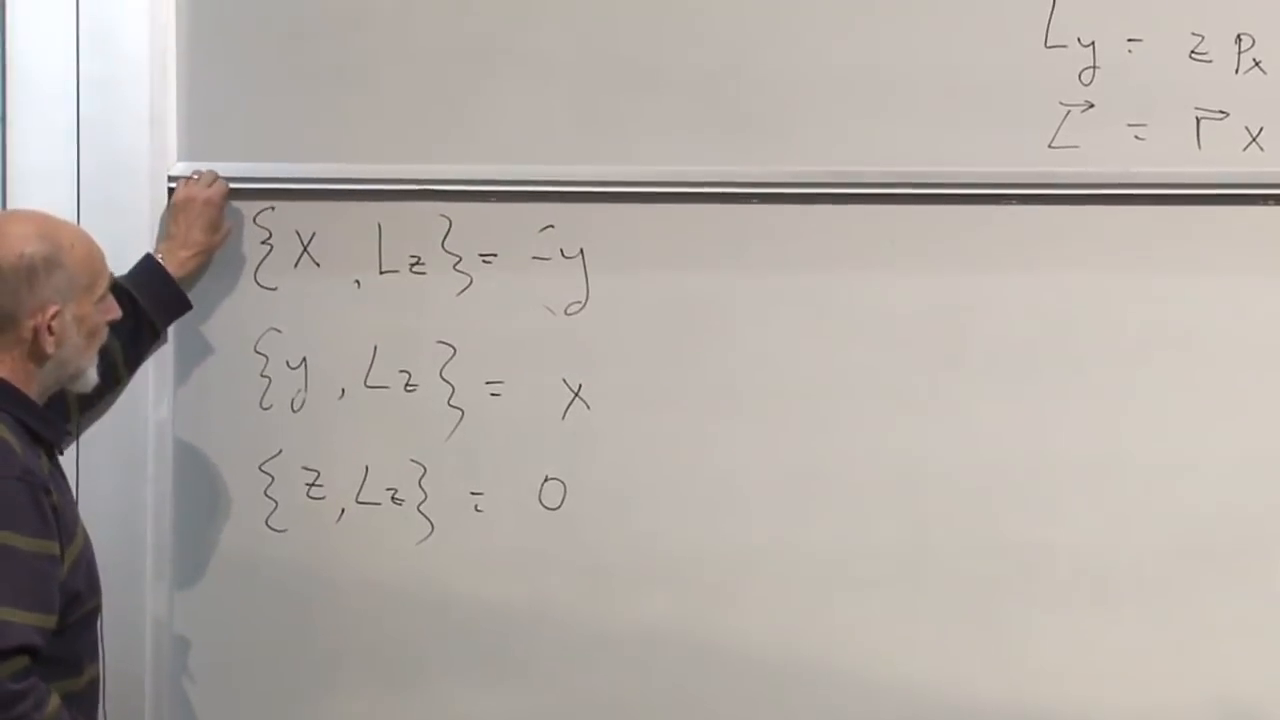
\includegraphics[width=0.82\textwidth]{lecture_08_figure_03.png}
  \caption{\(L_z\)との座標の括弧：この括弧は\((x,y,z)\)の無限小回転を再現する。}
  \lectureframe{00:38:41}
\end{figure}

運動量もまたベクトルであり、同じ計算により
\begin{equation}
  \begin{aligned}
    \{p_x,L_z\}&=-p_y,\\
    \{p_y,L_z\}&=p_x,\\
    \{p_z,L_z\}&=0.
  \end{aligned}
  \label{eq:l8-momentum-rotation-brackets}
\end{equation}
が得られる。

\begin{figure}[htbp]
  \centering
  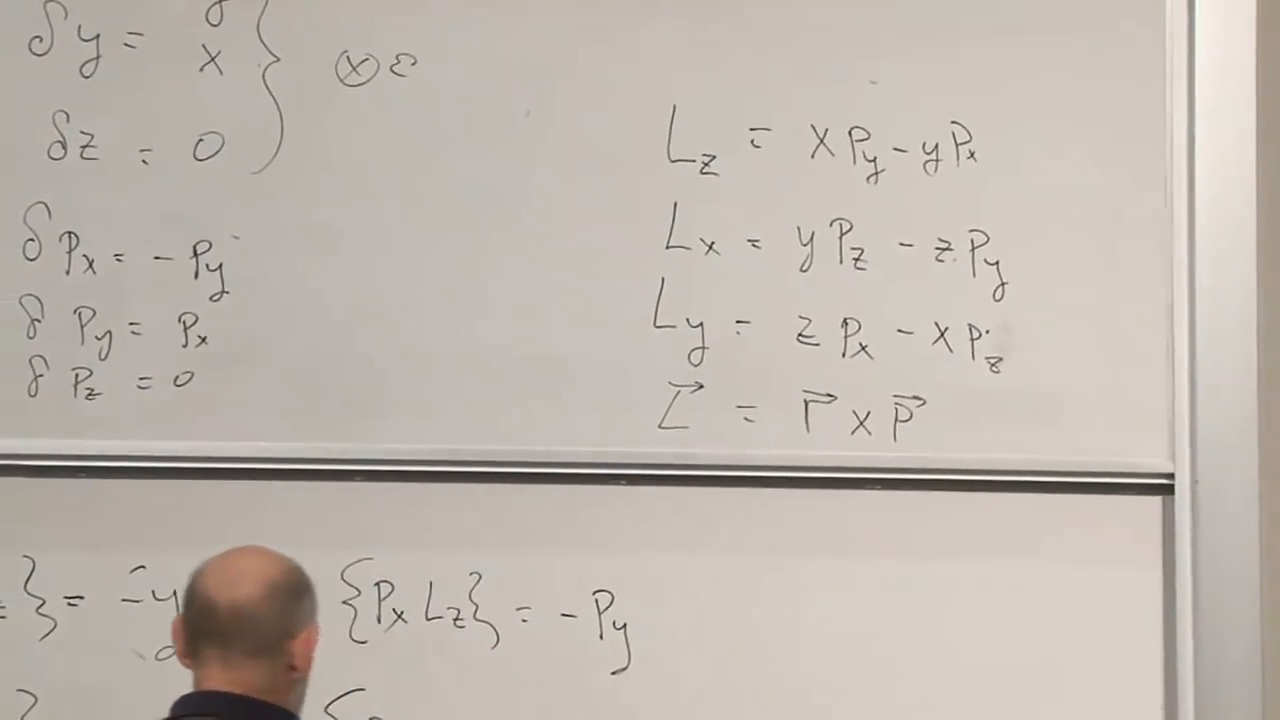
\includegraphics[width=0.82\textwidth]{lecture_08_figure_04.png}
  \caption{位置と運動量は、\(L_z\)が生成する回転の下で同じベクトルパターンに従って変換される。}
  \lectureframe{00:42:08}
\end{figure}

したがって、一般的なハミルトニアンによる言明は
\begin{equation}
  \boxed{\delta_G A=\epsilon\{A,G\}.}
  \label{eq:l8-generator-rule}
\end{equation}
である。相空間の任意の関数\(G\)はこのような無限小正準変換を定義する。\(G=L_z\)ならば、それは回転である。\(G=H\)ならば、それは時間の微小な進みである。

\begin{classroomqa}
  \audiencequestion{講義では系を回転させると言ったり、座標を回転させると言ったりすることがある。括弧の式ではどちらの規約が用いられているのか。\lecturetimestamp{00:28:22--00:29:35}}
  \lecturerresponse{式~\eqref{eq:l8-z-rotation}が規約を定めている。すなわち、無限小の能動的回転
  \((x,y)\mapsto(x-\epsilon y,y+\epsilon x)\)
  である。軸の受動的回転は逆の符号をもつ。ひとたび規約が定まれば、括弧の公式は曖昧さをもたない。}
\end{classroomqa}

\section{運動量が平行移動を生成する}

1つの座標における平行移動は
\begin{equation}
  \delta q=\epsilon.
  \label{eq:l8-q-translation}
\end{equation}
をもつ。ここで式~\eqref{eq:l8-noether-variation}において\(F(q)=1\)であるから、対応する保存量は\(p\)である。生成子についての主張は
\begin{equation}
  \{f(q),p\}=\frac{df}{dq}.
  \label{eq:l8-translation-derivative}
\end{equation}
を予測する。講義ではまずこれをべき乗について帰納法で証明する。基底の場合は
\(\{q,p\}=1\)
である。
\begin{equation}
  \{q^{n-1},p\}=(n-1)q^{n-2}.
  \label{eq:l8-induction-hypothesis}
\end{equation}
と仮定する。すると積の規則により
\begin{align}
  \{q^n,p\}
  &=\{q\,q^{n-1},p\}\\
  &=q\{q^{n-1},p\}+\{q,p\}q^{n-1}\\
  &=(n-1)q^{n-1}+q^{n-1}\\
  &=nq^{n-1}.
  \label{eq:l8-power-translation}
\end{align}
が得られる。線形性により、この結果は多項式および収束べき級数表示へ拡張される。より直接には、括弧の定義により、すべての微分可能な\(f(q)\)に対して式~\eqref{eq:l8-translation-derivative}が得られる：
\begin{equation}
  \{f(q),p\}
  =
  \frac{\partial f}{\partial q}
  \frac{\partial p}{\partial p}
  =f'(q).
\end{equation}

\begin{figure}[htbp]
  \centering
  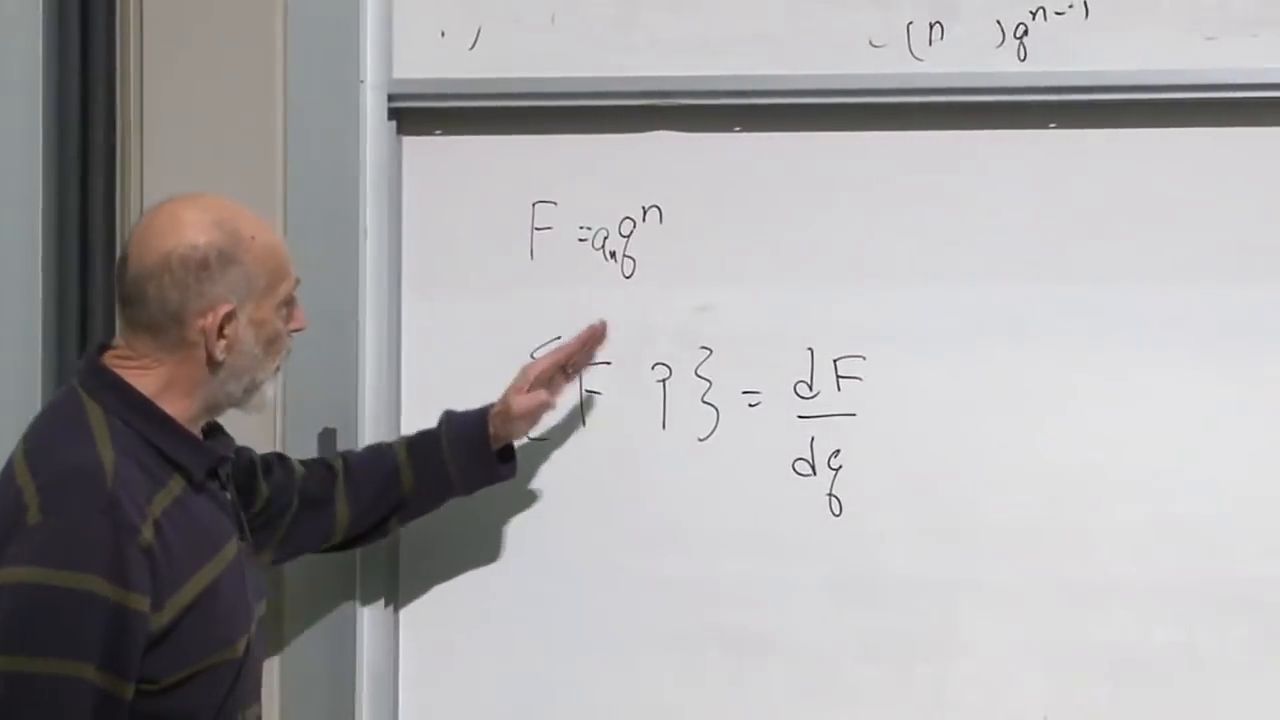
\includegraphics[width=0.82\textwidth]{lecture_08_figure_05.png}
  \caption{帰納法の議論の後の平行移動の結果：
  \(\{F(q),p\}=dF/dq\)。}
  \lectureframe{00:53:18}
\end{figure}

ここまでで、1つの考え方の3つの現れを見てきた：
\begin{center}
  \begin{tabular}{@{}>{\raggedright\arraybackslash}p{0.37\textwidth}
                      >{\raggedright\arraybackslash}p{0.55\textwidth}@{}}
    \toprule
    生成子と変換 & 無限小作用\\
    \midrule
    \(H\)、時間平行移動 & \(\delta_tA=\epsilon\{A,H\}\)\\
    \(p_i\)、空間平行移動 & \(\delta A=\epsilon\{A,p_i\}\)\\
    \(L_i\)、回転 & \(\delta A=\epsilon\{A,L_i\}\)\\
    \bottomrule
  \end{tabular}
\end{center}
連続対称性に対応する保存量は、その対称性の生成子でもある。

\section{1つの括弧、2つの読み方}

\(G(q,p)\) を提案された生成子とする。それが保存され、かつ陽に時間に依存しないならば、
\begin{equation}
  \dot G=\{G,H\}=0.
  \label{eq:l8-g-conserved}
\end{equation}
反対称性により、
\begin{equation}
  \{H,G\}=0.
  \label{eq:l8-h-invariant}
\end{equation}
これらの方程式は数学的に等価であるが、その物理的な読み方は異なる：
\begin{itemize}
  \item \(\{G,H\}=0\) は、\(G\) が \(H\) の生成する時間発展の下で変化しないことを述べている。
  \item \(\{H,G\}=0\) は、\(H\) が \(G\) の生成する変換の下で変化しないことを述べている。
\end{itemize}
第一は保存則であり、第二はハミルトニアンの対称性である。ネーターの関係は一つのゼロに圧縮されている。

\begin{figure}[htbp]
  \centering
  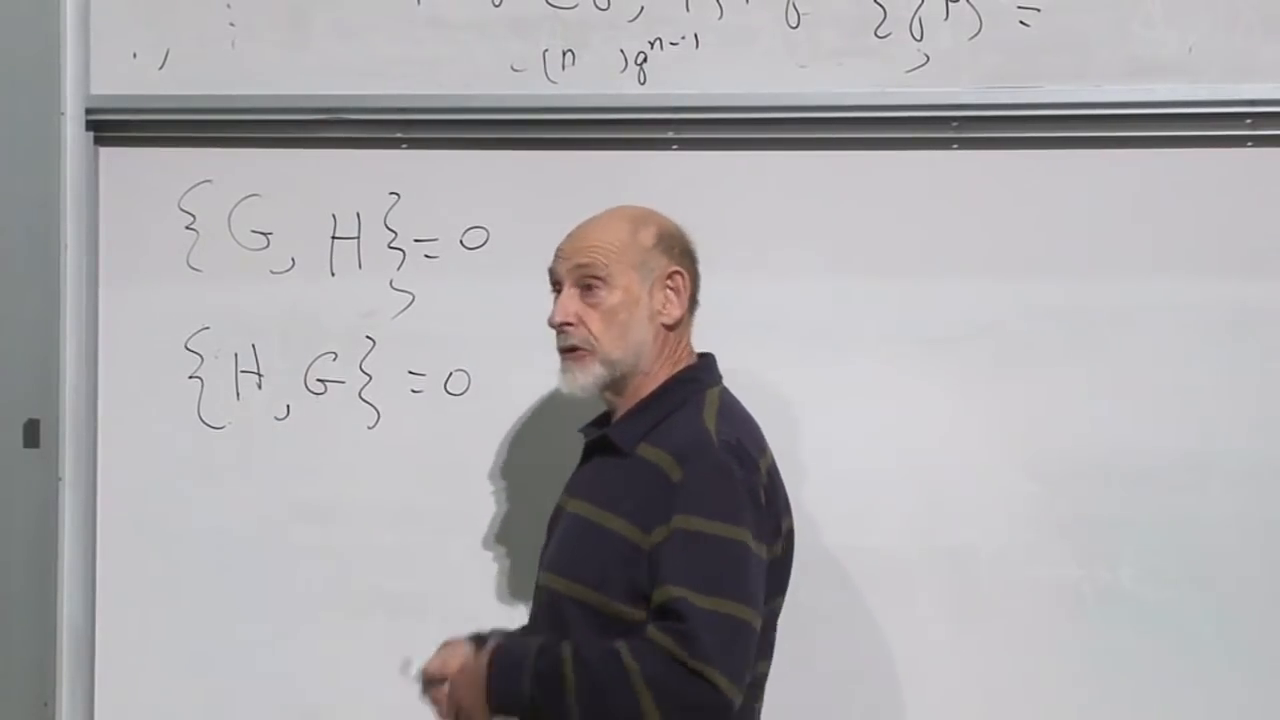
\includegraphics[width=0.82\textwidth]{lecture_08_figure_06.png}
  \caption{同じ消える括弧の二つの順序：\(G\) の保存と、\(G\) の生成する変換の下での \(H\) の不変性。}
  \lectureframe{01:03:05}
\end{figure}

\begin{classroomqa}
  \audiencequestion{保存量が既知であるとき、対応する対称性は常に復元できるか。\lecturetimestamp{01:01:42--01:02:15}}
  \lecturerresponse{このハミルトニアンの枠組みでは、できる。位相空間の各変数と \(G\) との括弧を取ればよい。その集まり
  \(\delta_GA=\epsilon\{A,G\}\) は変数がどのように変換するかを示す。例えば、\(L_z\) との括弧は、その解釈が前もって知られていなくても回転を明らかにする。より進んだ設定では大域的および境界上の微妙な問題が生じうるが、ここで用いられるのは局所的な無限小の言明である。}
\end{classroomqa}

\begin{classroomqa}
  \audiencequestion{それらの括弧の方程式は、保存則の原因となる物理的な運動を我々に教えるか。
  \lecturetimestamp{00:56:01--00:58:13}}
  \lecturerresponse{いいえ。それらは対称変換を同定するのであって、実際の軌道を同定するのではない。\(L_z\) の保存は回転対称性を示すが、粒子が円を描いて運動するとは述べていない。実際の時間発展は \(H\) によって生成される。別の生成子との括弧は、位相空間における別の変換の方向を記述する。}
\end{classroomqa}

\begin{classroomqa}
  \audiencequestion{すでに保存を仮定しない一般的な変換の言明はあるか。\lecturetimestamp{01:02:40--01:04:45}}
  \lecturerresponse{はい。式~\eqref{eq:l8-generator-rule} は、保存されるかどうかに関わらず、すべての関数 \(G\) に対して無限小変換を定義する。それが対称性となるのは、ハミルトニアンが不変であるときのみである：\(\{H,G\}=0\)。同じ条件を逆の順序で読めば、\(G\) が保存されることが言える。}
\end{classroomqa}

\section{角運動量代数}

次の計算により、あらゆる回転の問題で粒子座標を引きずり回すのをやめることができる。まず
\[
  L_x=yp_z-zp_y,\qquad
  L_z=xp_y-yp_x.
\]
\(\{L_x,L_z\}\) では、ほとんどの交差項はその添字が正準対をなさないため消える。生き残る縮約は
\begin{align}
  \{L_x,L_z\}
  &=\{yp_z-zp_y,xp_y-yp_x\}\\
  &=xp_z-zp_x\\
  &=-L_y.
  \label{eq:l8-lx-lz}
\end{align}
を与える。順序を逆にすると負号が除かれる。座標を巡回させると
\begin{equation}
  \boxed{\begin{aligned}
    \{L_x,L_y\}&=L_z,\\
    \{L_y,L_z\}&=L_x,\\
    \{L_z,L_x\}&=L_y.
  \end{aligned}}
  \label{eq:l8-angular-algebra}
\end{equation}
が得られる。添字記法では、
\begin{equation}
  \{L_i,L_j\}=\varepsilon_{ijk}L_k.
  \label{eq:l8-angular-algebra-index}
\end{equation}

\begin{figure}[htbp]
  \centering
  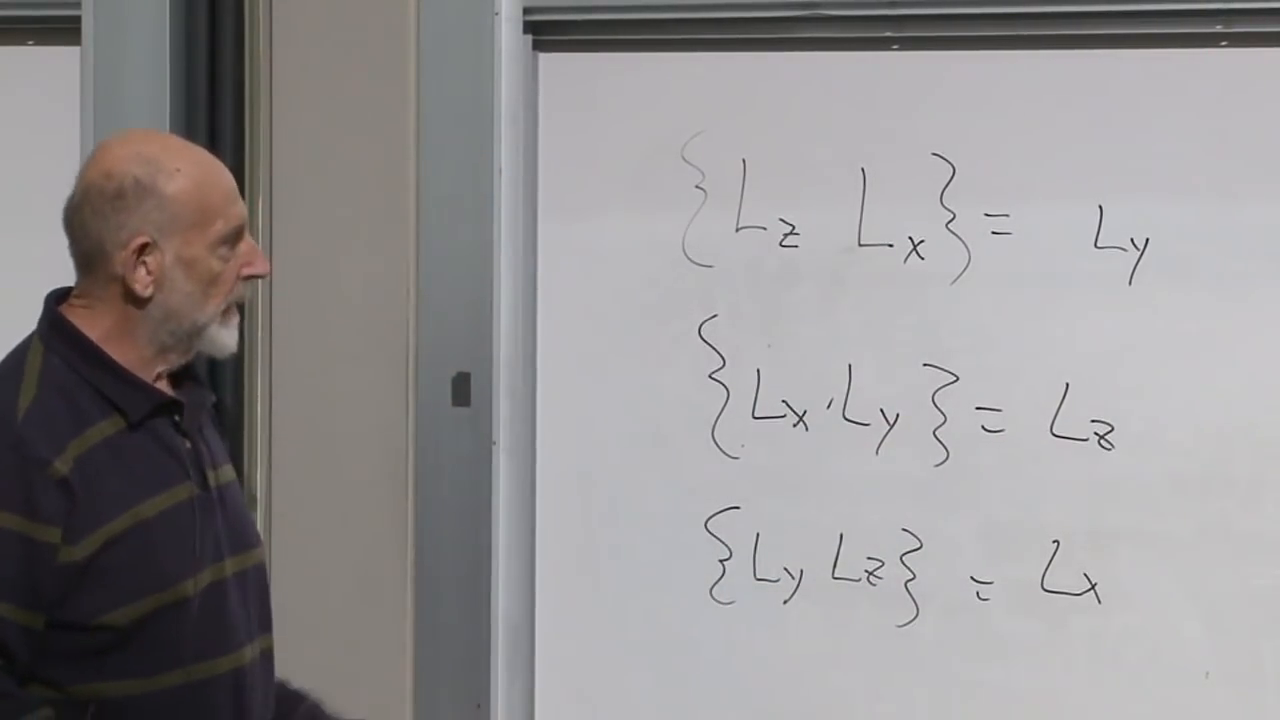
\includegraphics[width=0.82\textwidth]{lecture_08_figure_07.png}
  \caption{三つの角運動量成分の巡回的なポアソン括弧代数。}
  \lectureframe{01:10:52}
\end{figure}

この結果は予期することもできた。\(\boldsymbol L\) はベクトルであるから、その \(x\) 成分と \(L_z\) との括弧は、\(z\) 回転の下でのその成分の無限小変化、すなわち \(-L_y\) を与えなければならない。明示的な計算はこの幾何学的な議論を確認する。これらの方程式はまた、量子角運動量交換関係の古典的な先駆けでもある。

\section{高速ジャイロスコープ}

応用として、ジャイロスコープを考えよう。すなわち、中心が支点から固定距離 \(R\) にある高速で回転するはずみ車である。\(\boldsymbol r\) を支点から車輪の中心へ向かうものとする。はずみ車はその軸のまわりで非常に高速に回転するため、その支配的な角運動量はその方向に整列したままである。講義で用いられる近似では、
\begin{equation}
  \boldsymbol L=\ell\,\boldsymbol r,
  \qquad
  L_z=\ell z,
  \label{eq:l8-L-parallel-r}
\end{equation}
ここで \(\ell=L/R\) は定数として扱われる。章動や軸の運動に伴うより小さな角運動量は、まず無視される。

\begin{figure}[htbp]
  \centering
  \begin{tikzpicture}[scale=0.95,>=Latex]
    \coordinate (P) at (0,3.2);
    \coordinate (C) at (3.7,1.55);
    \draw[->] (0,-0.2) -- (0,4.35) node[above] {\(z\)};
    \fill (P) circle (1.7pt) node[left] {pivot};
    \draw[very thick,->] (P) -- (C)
      node[midway,above right] {\(\boldsymbol r\parallel\boldsymbol L\)};
    \fill (C) circle (1.7pt);
    \draw[dashed] (P) -- (0,1.55);
    \draw[dashed] (0,1.55) -- (C);
    \node[left] at (0,1.55) {\(z\)};
    \begin{scope}[shift={(C)},rotate=-24]
      \draw[very thick] (0,0) ellipse (0.65 and 1.35);
      \draw[thick] (0,0) ellipse (0.42 and 0.9);
    \end{scope}
    \draw[->,thick] (2.15,2.85)
      arc[start angle=140,end angle=35,radius=1.65];
  \end{tikzpicture}
  \caption{高速ジャイロスコープ近似。支点から中心までの距離は固定され、支配的なスピン角運動量は軸および \(\boldsymbol r\) に整列したままである。}
\end{figure}

\begin{figure}[htbp]
  \centering
  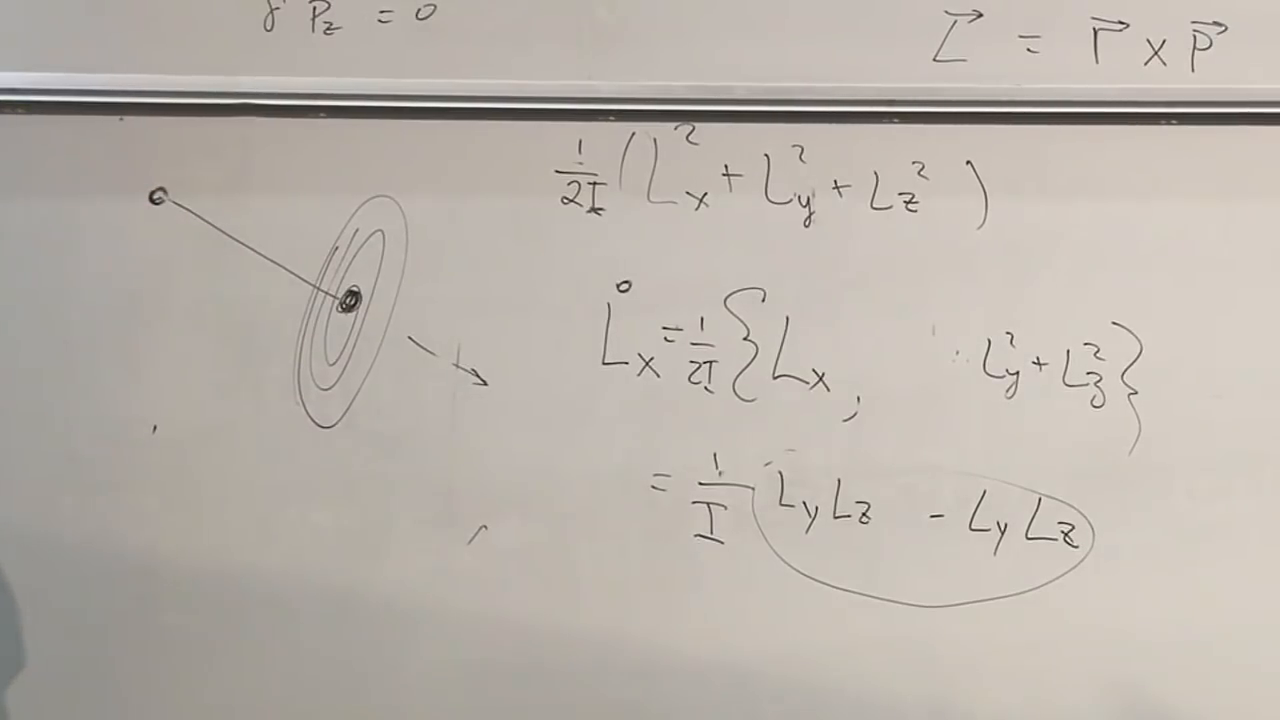
\includegraphics[width=0.82\textwidth]{lecture_08_figure_08.png}
  \caption{はずみ車の板書スケッチ、\(H_{\rm rot}=L^2/(2I)\)、および \(\boldsymbol L\) のトルクのない保存を証明する相殺。}
  \lectureframe{01:18:54}
\end{figure}

\subsection{重力なし：なぜ各成分が固定されたままであるか}

簡略化された軸対称回転子に対して、
\begin{equation}
  H_{\mathrm{rot}}
  =\frac{1}{2I}
  \left(L_x^2+L_y^2+L_z^2\right)
  =\frac{L^2}{2I}.
  \label{eq:l8-rotational-hamiltonian}
\end{equation}
係数は\(1/(2I)\)であり、\(I/2\)ではない。この間違いは黒板でなされ、訂正される。式~\eqref{eq:l8-angular-algebra}を用いると、
\begin{align}
  \dot L_x
  &=\{L_x,H_{\mathrm{rot}}\}\\
  &=\frac{1}{2I}\left(
    2L_y\{L_x,L_y\}
    +2L_z\{L_x,L_z\}
  \right)\\
  &=\frac{1}{I}\left(L_yL_z-L_zL_y\right)=0.
  \label{eq:l8-free-lx}
\end{align}
巡回的に、
\begin{equation}
  \dot L_x=\dot L_y=\dot L_z=0.
  \label{eq:l8-free-angular-momentum}
\end{equation}
スカラー\(L^2\)は各成分\(L_i\)との括弧がゼロである。この代数の言葉では、それはカシミールである。したがって、トルクのないジャイロスコープは角運動量の大きさと方向の両方を保つ。

\begin{classroomqa}
  \audiencequestion{ここで慣性モーメントは単なる数ですか？
  \lecturetimestamp{01:14:23--01:15:05}}
  \lecturerresponse{この簡約モデルでは、はい。それは車輪のスピン軸周りの質量分布を符号化する。一般の剛体は慣性モーメントテンソルと主軸における回転ハミルトニアン
  \(\sum_i L_i^2/(2I_i)\)を持つ。講義では、完全な剛体力学を展開するのではなく、ポアソン括弧法を示すことを目的としているため、より単純な高速対称回転子を選ぶ。}
\end{classroomqa}

\subsection{重力とポテンシャルの符号}

鉛直座標\(z\)を上向きに正とし、支点を原点に置く。車輪中心の重力ポテンシャルエネルギーは
\begin{equation}
  V=Mgz.
  \label{eq:l8-mgz}
\end{equation}
\(L_z=\ell z\)なので、
\begin{equation}
  V=cL_z,
  \qquad
  c=\frac{Mg}{\ell}=\frac{MgR}{L}.
  \label{eq:l8-potential-lz}
\end{equation}
ここで\(\boldsymbol L\)が\(\boldsymbol r\)に平行に選ばれるとき\(c>0\)である。フライホイールが逆方向に回転する場合、\(\boldsymbol L\)と\(\boldsymbol r\)の間の符号付き関係は逆転し、対応する符号付き歳差周波数も逆転する。

\begin{figure}[htbp]
  \centering
  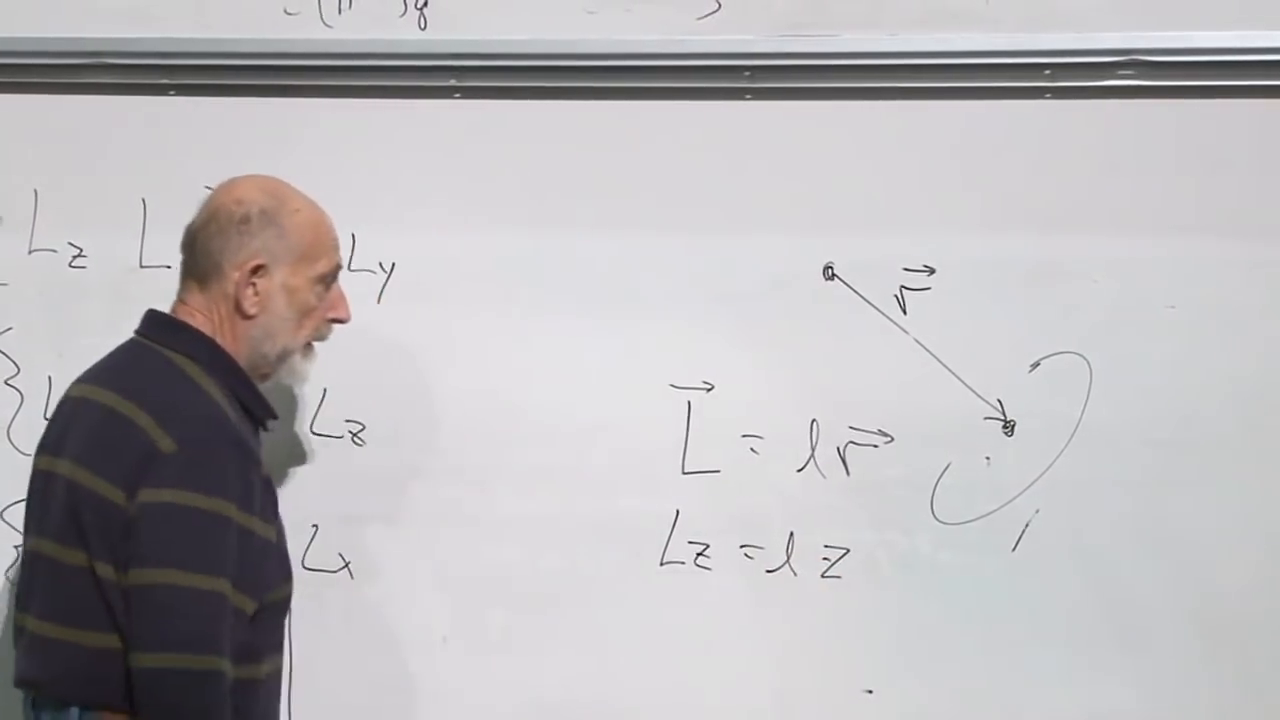
\includegraphics[width=0.82\textwidth]{lecture_08_figure_09.png}
  \caption{\(\boldsymbol L=\ell\boldsymbol r\)と\(L_z=\ell z\)の背後にある固定長の幾何学。}
  \lectureframe{01:25:38}
\end{figure}

\begin{figure}[htbp]
  \centering
  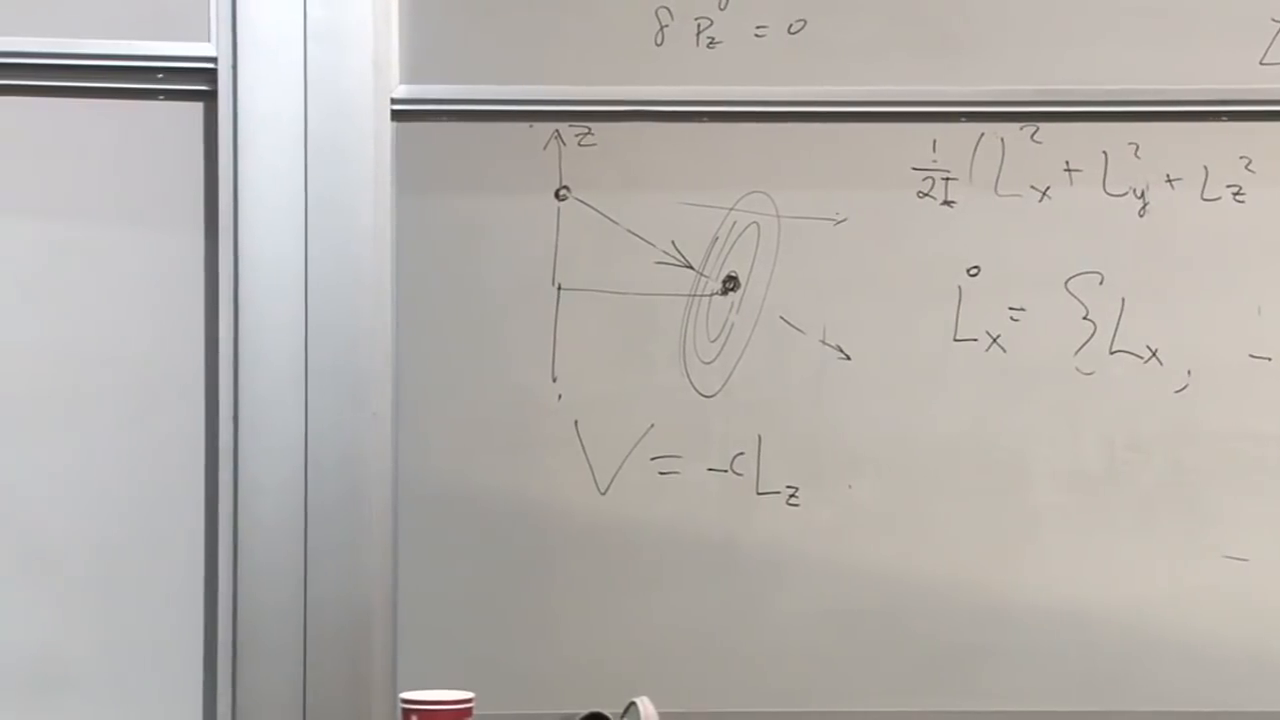
\includegraphics[width=0.82\textwidth]{lecture_08_figure_10.png}
  \caption{中間の黒板状態は\(V=-cL_z\)を示す。符号は後に\(z\)が上向きと固定された後で訂正される。\(\boldsymbol L=\ell\boldsymbol r\)と\(\ell>0\)で、整合する結果は
  \(V=+cL_z\)である。}
  \lectureframe{01:22:43}
\end{figure}

\begin{classroomqa}
  \audiencequestion{なぜ高さを角運動量の成分で置き換えてよいのですか？斜めの線は車軸ですか、それとも位置ベクトルですか？
  \lecturetimestamp{01:22:20--01:25:43}}
  \lecturerresponse{斜めの線は\(\boldsymbol r\)、すなわち固定支点から車輪中心へのベクトルとラベル付けするのが最善である。物理的な車軸がそれに沿って存在してもよいが、計算で用いられる関係は高速スピン近似
  \(\boldsymbol L=\ell\boldsymbol r\)である。したがってそれらの\(z\)成分は比例する。ライブ討論では、この区別に落ち着くまでにラベルが何度か変わる。}
\end{classroomqa}

\begin{classroomqa}
  \audiencequestion{どのような仮定が\(\ell\)を定数にするのか、そして車輪中心が半径方向に滑ることができるなら何が破綻するのか？
  \lecturetimestamp{01:25:43--01:26:38,\allowbreak\ 01:34:22--01:35:00}}
  \lecturerresponse{支配的なスピンは遅い運動に伴う角運動量よりはるかに大きいと仮定され、支点から中心までの距離は固定されている。するとスピンの大きさはほとんど変化せず、\(\boldsymbol L\)は\(\boldsymbol r\)とともに回転する。もし中心が半径方向に滑ることができるなら、\(z\)はもはや一つの定数係数で\(L_z\)に比例しなくなり、簡約ハミルトニアン\(V=cL_z\)は運動を記述しないであろう。}
\end{classroomqa}

\begin{classroomqa}
  \audiencequestion{なぜ黒板は最初にマイナス符号を示し、後にプラス符号を示すのですか？スピンの向きは重要ですか？
  \lecturetimestamp{01:27:13--01:28:15,\allowbreak\ 01:33:09--01:33:21}}
  \lecturerresponse{最初の符号は、未確定の軸の規約が混ざったライブ黒板の誤りである。\(z\)が上向きと定義されると、\(V=Mgz\)は高さとともに増加する。\(\boldsymbol L=\ell\boldsymbol r\)で\(\ell>0\)なら、これは
  \(V=+cL_z\)を与える。スピンを逆にすると符号付き比例関係と歳差の向きが逆転するが、任意の符号選択が復活するわけではない。}
\end{classroomqa}

\subsection{三つの短い方程式からの歳差}

完全な簡約ハミルトニアンは
\begin{equation}
  H=
  \frac{1}{2I}\left(L_x^2+L_y^2+L_z^2\right)+cL_z.
  \label{eq:l8-full-gyro-hamiltonian}
\end{equation}
\(L^2\)がすべての\(L_i\)とゼロ括弧を持つことはすでに示した。線形項のみが寄与する：
\begin{align}
  \dot L_z&=\{L_z,H\}=0,\\
  \dot L_x&=\{L_x,H\}=c\{L_x,L_z\}=-cL_y,\\
  \dot L_y&=\{L_y,H\}=c\{L_y,L_z\}=cL_x.
  \label{eq:l8-precession-equations}
\end{align}

\begin{figure}[htbp]
  \centering
  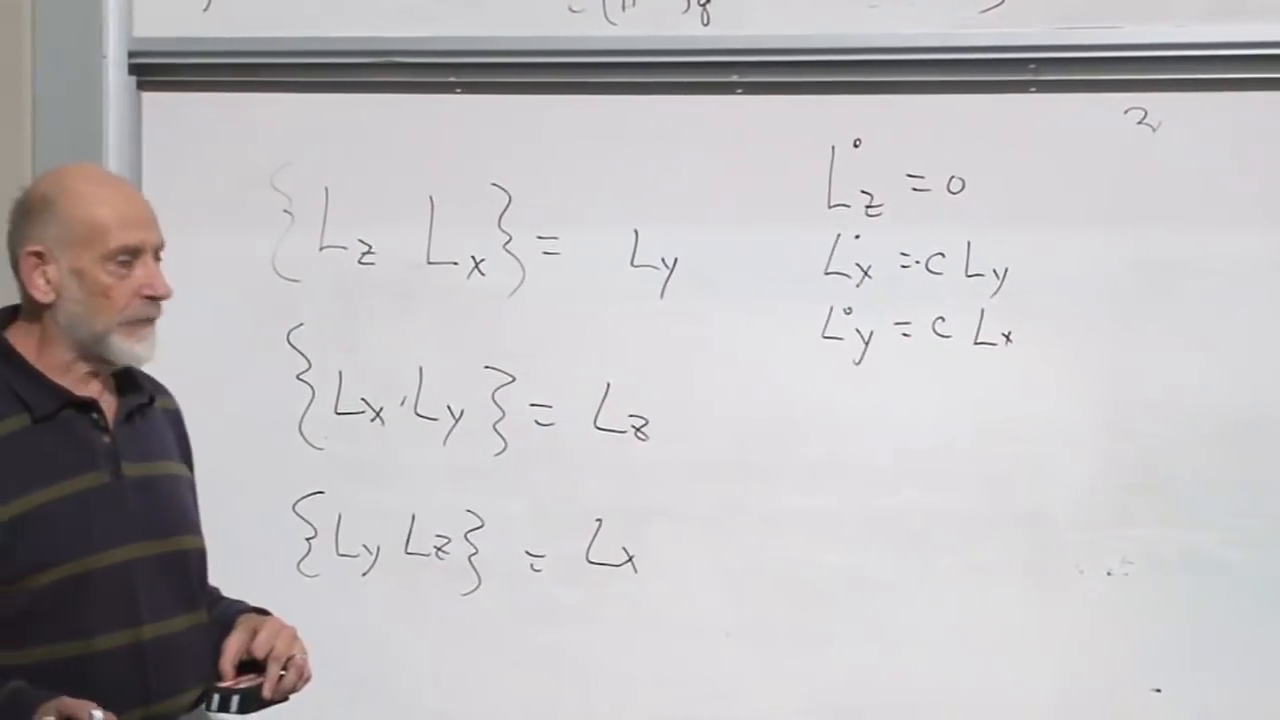
\includegraphics[width=0.82\textwidth]{lecture_08_figure_11.png}
  \caption{最終的な成分方程式：\(L_z\)は定数であり、\(L_x\)と\(L_y\)は互いに回転し合う。}
  \lectureframe{01:30:35}
\end{figure}

鉛直成分と水平方向の大きさは一定である：
\begin{equation}
  \frac{d}{dt}(L_x^2+L_y^2)
  =2L_x(-cL_y)+2L_y(cL_x)=0.
\end{equation}
水平成分を組み合わせると、
\begin{equation}
  L_+=L_x+iL_y,
  \qquad
  \dot L_+=icL_+,
\end{equation}
したがって
\begin{equation}
  L_+(t)=L_+(0)e^{ict}.
  \label{eq:l8-precession-solution}
\end{equation}
よって角運動量ベクトルは鉛直軸の周りを角速度\(|c|=MgR/L\)で歳差運動する。この理想化された定常運動では、その傾きは固定されたままである。

\begin{classroomqa}
  \audiencequestion{歳差方程式を書くとき、回転エネルギー項は無視されたのですか？
  \lecturetimestamp{01:35:01--01:35:49}}
  \lecturerresponse{いいえ。それは式~\eqref{eq:l8-full-gyro-hamiltonian}のように完全なハミルトニアンに属する。\(\{L_i,L^2\}=0\)なので\(\dot L_i\)への寄与は単にゼロである。これはトルクのない計算ですでに証明された相殺である。学生の質問がこの暗黙のステップを明示的にする。}
\end{classroomqa}

\begin{classroomqa}
  \audiencequestion{一様な歳差運動は平衡なのか。小さな蹴りを与えた後、何が起こるのか。\lecturetimestamp{01:32:38--01:33:08}}
  \lecturerresponse{静的平衡というよりは、定常運動または停留運動と呼ぶ方が適切である。小さな蹴りは一般に章動、すなわち傾斜角の振動を付加する。非常に速く回転する車輪ではその振動は小さく、それゆえ簡約された取り扱いではほぼ一様な歳差運動のみを保持する。}
\end{classroomqa}

\begin{classroomqa}
  \audiencequestion{歳差運動には支持体または実際の軸が必要なのか。\lecturetimestamp{01:31:49--01:32:38,\allowbreak\ 01:33:49--01:35:00}}
  \lecturerresponse{この力学模型は支点から中心までの距離が固定されていると仮定しているので、何らかの拘束が支持を与えている。より深い代数的結果はもっと広い。角運動量が一つの成分について線形なハミルトニアン項をもつときはいつでも、同じ括弧代数が歳差運動を生み出す。角運動量の微視的起源は、軸に取り付けられた文字通りの車輪である必要はない。}
\end{classroomqa}

\begin{classroomqa}
  \audiencequestion{これは磁場中の電子スピンや核スピンの歳差運動、あるいは惑星軌道の歳差運動と同じものか。\lecturetimestamp{01:35:50--01:37:00}}
  \lecturerresponse{磁場に結合した磁気モーメントはスピン成分について線形なハミルトニアンをもち、したがって同じ角運動量代数に従う。核スピンの歳差運動は核磁気共鳴の基礎である。惑星軌道の近日点の歳差運動は、たまたま\emph{歳差運動}という語を共有する別の現象であり、同じ計算ではない。}
\end{classroomqa}

\begin{classroomqa}
  \audiencequestion{横付けのジャイロスコープは本質的に回転独楽と同じ物体か。\lecturetimestamp{01:37:02--01:37:23}}
  \lecturerresponse{はい。区別は主に幾何学的な言葉遣いである。回転軸が支持体から横向きに伸びているときは通常ジャイロスコープと言い、ほぼ鉛直であるときは独楽と言う。角運動量とトルクの構造は同じである。}
\end{classroomqa}

\section{計算が成し遂げたこと}

オイラー角は導入されず、車輪の各部分ごとの座標が追跡されることもなかった。一旦
\[
  \{L_i,L_j\}=\varepsilon_{ijk}L_k
\]
が分かれば、関心のある変数の方程式は直接に導かれた。これが意図された威力の実証である。振動子は、ポアソン括弧が馴染み深い力学を再現できることを示した。角運動量は、それらがはるかに多くを行うことを示した：
\begin{itemize}
  \item 保存量はその関連する無限小対称性を生成する；
  \item \(G\)の保存と\(H\)の不変性は
  \(\{G,H\}=0\)の二つの読み方である；
  \item 観測量の代数はそれ自身で閉じることができ、微視的座標に戻ることなく力学を解くことを可能にする；
  \item 一つの角運動量成分について線形なハミルトニアンは、その軸の周りの歳差運動を生み出す。
\end{itemize}
講義は一般の剛体に対する完全なオイラー方程式の手前で止まる。そのより狭い結論はすでに完結している：正しい生成子とそれらのポアソン代数は、驚くべき経済性で対称性と運動の両方を明らかにする。